% Change figure labeling to section and #
\renewcommand\thefigure{\thesection.\arabic{figure}}   

\clearpage
\section{Appendices}
  \subsection{Data Dictionary}
    \subsubsection{Actor Descriptions}

App users will be the primary actors of the application and they will generally fit into the same category. Users will want to interface with the application to allow it to pull their transaction history from the blockchain so that they can categorize their data. Professional financial management entities could conceivably use data created from our software and if time permits we will implement data formatting to work in conjunction with popular financial planning systems and software. 

Users will supply their information, such as bitcoin addresses and spending categories, this will allow them to graph their data, maintain balances, and users will also be able to delete all of their own data. 

Individuals who own and spend bitcoin will be most interested in using our app. Financial management and planning is an important part of financial responsibilty and a ledger to report spending habits will be of use to many members of the bitcoin community.

Support and maintenance of the system is mostly the users responsibility. Maintaining the hardware is the responsibility of the user, maintaining the operating system and related libraries will be the responsibility of Google and the phone manugacturer. Maintaining the software will primarily be done by Prestige Worldwide while any sub libraries and related software support will be maintained by their software development teams.

The system will use blockchain APIs provided by a number of providers. Many of the APIs are free and there is even an option to run our own server, utilizing open source software to interface with the blockchain and provide API services to our app users. Final design and implementation will be decided on time to implement and performance to the user metric.

No other systems will be dependent on our app. Therefore no functionality is critical for any downstream applications.

\clearpage
  \subsubsection{Use Case Descriptions}

  
  %-----------------------------------------------
  % Use case 3.5 : Aggreate Wallet View
  %-----------------------------------------------

  \begin{figure}[H]
    \centering
    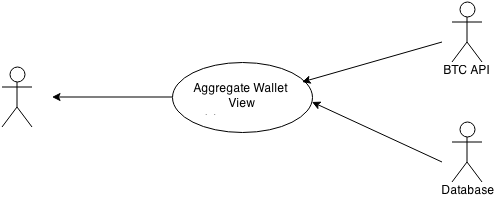
\includegraphics[scale=0.6]{../diagrams/usecase_3_5.png}
    \caption{Managing User Wallets}
  \end{figure}

  % -- Use Case : Aggreate Wallet View
  \begin{table}[H]
    \centering
    \resizebox{0.8\columnwidth}{!}{%
    \tabulinesep=1.2mm
    \rowcolors{2}{gray!25}{white}
    \begin{tabu}{| r | X |}
      \rowfont{\color{black}}
      \taburulecolor{black}
      \hline
      \taburowcolors 1{green .. green}
      \multicolumn{2}{|l|}{\textbf{\textsf{WalleTx: Aggregate Wallet View}}}\\
      \hline

      \taburowcolors 2{light-gray .. white}
      Actors & User, SQLite Database, Blockchain API\\
      Description & User will view an aggregate view of all imported wallets that contains the total balance and number of transactions\\
      Data & all imported wallets, transaction hashes, and total balance of combined wallets\\
      Stimulus & User initiated option\\
      Response & Summary view for all wallets will be displayed showing a list of all imported wallets, total balance and number of transactions.\\
      Comments & \\

      \taburowcolors 1{green .. green}
      \multicolumn{2}{|l|}{\textbf{\textsf{\footnotesize{Figure 7.7}}}}\\
      \hline
    \end{tabu}%
  }
  \end{table}
  \clearpage 
  
  %-----------------------------------------------
  % Use case 3.1 : Managing User Wallets
  %-----------------------------------------------

  \begin{figure}[H]
    \centering
    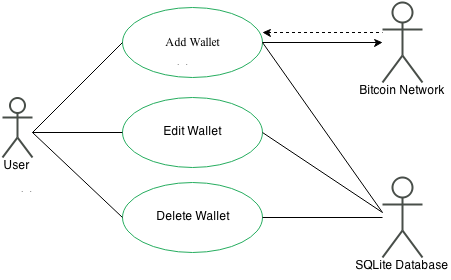
\includegraphics[scale=0.6]{../diagrams/usecase_3_1.png}
    \caption{Managing User Wallets}
  \end{figure}

  % -- Use Case : Add Wallet
  \begin{table}[H]
    \centering
    \resizebox{0.8\columnwidth}{!}{%
    \tabulinesep=1.2mm
    \rowcolors{2}{gray!25}{white}
    \begin{tabu}{| r | X |}
      \rowfont{\color{black}}
      \taburulecolor{black}
      \hline
      \taburowcolors 1{green .. green}
      \multicolumn{2}{|l|}{\textbf{\textsf{WalleTx: Add Wallet}}}\\
      \hline

      \taburowcolors 2{light-gray .. white}
      Actors & User, SQLite Database, Blockchain API\\
      Description & User will add an existing wallet public key to the application to enable mapping of transactions to the wallet public address\\
      Data & public wallet address, transaction hashes, tags associate with transactions\\
      Stimulus & User initiated option\\
      Response & Additional view will open up allowing the user to manual type their wallet address, paste from the clipboard, or scan a qr code. After a valid bitcoin public address is entered the application will contact the Blockchain.info API to pull transaction information putting that information into the database. View will return to the main wallet view.\\
      Comments & \\

      \taburowcolors 1{green .. green}
      \multicolumn{2}{|l|}{\textbf{\textsf{\footnotesize{Figure 7.8}}}}\\
      \hline
    \end{tabu}%
  }
  \end{table}

  % -- Use Case : Modify Wallet
  \begin{table}[H]
    \centering
    \resizebox{0.8\columnwidth}{!}{%
    \tabulinesep=1.2mm
    \rowcolors{2}{gray!25}{white}
    \begin{tabu}{r | X}
      \rowfont{\color{black}}
      \taburulecolor{black}

      \taburowcolors 1{green .. green}
      \multicolumn{2}{l}{\textbf{\textsf{WalleTx: Modify Wallet}}}\\
      \hline

      \taburowcolors 2{light-gray .. white}
      Actors & User, SQLite Database\\
      Description & User will be able to edit the name of the wallet.\\
      Data & Public Wallet Address associated with database entries\\
      Stimulus & User initiated option\\
      Response & View will open allowing the user to change the name of the wallet.\\
      Comments & Changing the wallet address would only serve to change all the underlying transactions, therefore it may be a better idea to only allow adding or removing public wallet addresses to manipulate public wallet address data in the database. Other features not implemented by the Bitcoin blockchain, such as currency pair, wallet nickname, etc. can be modified here.\\
      \taburowcolors{green .. green}
      \multicolumn{2}{|l|}{\textbf{\textsf{\footnotesize{Figure 7.8}}}}\\

    \end{tabu}%
  }
  \end{table}

  % -- Use Case : Remove Wallet
  \begin{table}[H]
    \tabulinesep=1.2mm
    \centering
    \resizebox{0.8\columnwidth}{!}{%
    \rowcolors{2}{gray!25}{white}
    \begin{tabu}{r | X}
      \rowfont{\color{black}}
      \taburulecolor{black}

      \taburowcolors 1{green .. green}
      \multicolumn{2}{l}{\textbf{\textsf{WalleTx: Remove Wallet}}}\\
      \hline

      \taburowcolors 2{light-gray .. white}
      Actors & User, SQLite Database\\
      Description & User will remove an existing wallet public key from the application and have corresponding data removed from the SQLite database.\\
      Data & public wallet address\\
      Stimulus & User initiated option\\
      Response & Dialog will pop up allowing the user to confirm (possibly have a text input required to continue) and when confirmed the data will be purged from the database.\\
      Comments & \\
      \taburowcolors{green .. green}
      \multicolumn{2}{|l|}{\textbf{\textsf{\footnotesize{Figure 7.8}}}}\\

    \end{tabu}%
  }
  \end{table}

  %-----------------------------------------------
  % Use case 3.2 : Managing wallet groups
  %-----------------------------------------------
\begin{figure}[H]
    \centering
    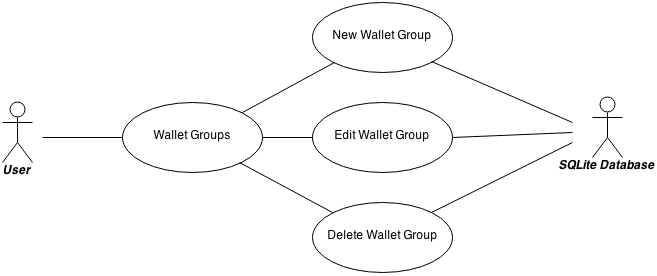
\includegraphics[scale=0.6]{../diagrams/usecase_3_2.png}
    \caption{Managing Wallet Groups}
  \end{figure}
  
  % -- Use Case 3.2 : View all wallet groups 
  \begin{table}[H]
    \tabulinesep=1.2mm
    \centering
    \resizebox{0.8\columnwidth}{!}{%
    \rowcolors{2}{gray!25}{white}
    \begin{tabu}{r | X}
      \rowfont{\color{black}}
      \taburulecolor{black}
      \taburowcolors 1{green .. green}
      \multicolumn{2}{l}{\textbf{\textsf{WalleTx: View all transaction tag categories}}}\\
      \hline
      \taburowcolors 2{light-gray .. white}
      Actors & 
        User, SQLite Database\\
      Description & 
        User is presented with a list view of wallet groups with options to: (1) Add a new wallet group, (2) Edit a wallet group, and (3) Delete a wallet group\\
      Data & 
        Wallet group categories\\
      Stimulus & 
        User initiated option. User selects Wallet Groups from the menu\\
      Response & 
        Application opens CRUDGroupActivity and populates the list view with all the groups in the group table\\
      Comments & 
        This is entry point for user to add, edit and delete wallet groups\\
      \taburowcolors 1{green .. green}
      \multicolumn{2}{|l|}{\textbf{\textsf{\footnotesize{Figure 7.9}}}}\\
      \hline
    \end{tabu}%
  }
  \end{table}

  % -- Use Case 3.2.2 : Add New Wallet Group 
  \begin{table}[H]
    \tabulinesep=1.2mm
    \centering
    \resizebox{0.8\columnwidth}{!}{%
    \rowcolors{2}{gray!25}{white}
    \begin{tabu}{r | X}
      \rowfont{\color{black}}
      \taburulecolor{black}
      \taburowcolors 1{green .. green}
      \multicolumn{2}{l}{\textbf{\textsf{WalleTx: Add wallet group category}}}\\
      \hline
      \taburowcolors 2{light-gray .. white}
      Actors & 
        User, SQLite Database\\
      Description & 
        User adds a new wallet group (by name) to the application\\
      Data & 
        Wallet group name\\
      Stimulus & 
        User initiated option\\
      Response & 
        A dialog will open containing: (1) a text field for entering the new wallet group, (2) a Cancel button, (3) and an Add button. If Add is selected, user entered wallet group name is inserted into the Wallet Group table and user is returned to the CRUDGroupActivity. If cancel is selected, user is returned to the CRUDGroupActivity.\\
      Comments & 
        Response should validate for empty wallet group name. CRUDGroupActivity UI must be updated upon successful insertion of a new tag category\\
      \taburowcolors 1{green .. green}
      \multicolumn{2}{|l|}{\textbf{\textsf{\footnotesize{Figure 7.9}}}}\\
      \hline
    \end{tabu}%
  }
  \end{table}

  % -- Use Case 3.2.3 : Edit Wallet Group
  \begin{table}[H]
    \tabulinesep=1.2mm
    \centering
    \resizebox{0.8\columnwidth}{!}{%
    \rowcolors{2}{gray!25}{white}
    \begin{tabu}{r | X}
      \rowfont{\color{black}}
      \taburulecolor{black}
      \taburowcolors 1{green .. green}
      \multicolumn{2}{l}{\textbf{\textsf{WalleTx: Edit wallet group category}}}\\
      \hline
      \taburowcolors 2{light-gray .. white}
      Actors & 
        User, SQLite Database\\
      Description & 
        User edits an existing wallet group\\
      Data & 
        Wallet group name\\
      Stimulus & 
        User initiated option. User selects edit button from wallet group view.\\
      Response & 
        A dialog will open containing: (1) an edit text field for updating wallet group, (2) a Cancel button, (3) and an Edit button. If Edit is selected, the wallet group is updated in the Wallet Group table and user is returned to the CRUDGroupActivity. If cancel is selected, user is returned to the CRUDGroupActivity.\\
      Comments & 
        Response should validate for empty wallet group name. CRUDGroupActivity UI must be updated upon successful update of a tag category\\
      \taburowcolors 1{green .. green}
      \multicolumn{2}{|l|}{\textbf{\textsf{\footnotesize{Figure 7.9}}}}\\
      \hline
    \end{tabu}%
  }
  \end{table}

  % -- Use Case 3.2.4 : Delete wallet group
  \begin{table}[H]
    \tabulinesep=1.2mm
    \centering
    \resizebox{0.8\columnwidth}{!}{%
    \rowcolors{2}{gray!25}{white}
    \begin{tabu}{r | X}
      \rowfont{\color{black}}
      \taburulecolor{black}
      \taburowcolors 1{green .. green}
      \multicolumn{2}{l}{\textbf{\textsf{WalleTx: Delete Wallet Group}}}\\
      \hline
      \taburowcolors 2{light-gray .. white}
      Actors & 
        User, SQLite Database\\
      Description & 
        User deletes an existing wallet group\\
      Data & 
        Wallet group name\\
      Stimulus & 
        User initiated option. User selects delete button from wallet group list view.\\
      Response & 
        A dialog will open confirming if user wishes to delete the wallet group. If confirmed, the wallet group must be removed then reassign all wallets associated with deleted group to the default group and then removed from the Wallet Group table. User is then returned to the CRUDGroupActivity.\\
      Comments & 
        CRUDGroupActivity UI must be updated upon successful update of the wallet groups\\
      \taburowcolors 1{green .. green}
      \multicolumn{2}{|l|}{\textbf{\textsf{\footnotesize{Figure 7.9}}}}\\
      \hline
    \end{tabu}%
  }
  \end{table}
  
  
  %-----------------------------------------------
  % Use case 3.3 : Managing tx tag categories
  %-----------------------------------------------

  \begin{figure}[H]
    \centering
    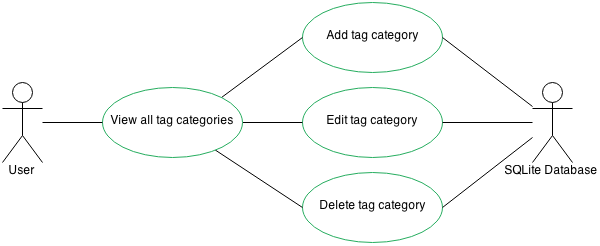
\includegraphics[scale=0.6]{../diagrams/usecase_3_3.png}
    \caption{Managing Transaction Tag Categories}
  \end{figure}

  % -- Use Case 3.3 : View all tag categories
  \begin{table}[H]
    \tabulinesep=1.2mm
    \centering
    \resizebox{0.8\columnwidth}{!}{%
    \rowcolors{2}{gray!25}{white}
    \begin{tabu}{r | X}
      \rowfont{\color{black}}
      \taburulecolor{black}
      \taburowcolors 1{green .. green}
      \multicolumn{2}{l}{\textbf{\textsf{WalleTx: View all transaction tag categories}}}\\
      \hline
      \taburowcolors 2{light-gray .. white}
      Actors & 
        User, SQLite Database\\
      Description & 
        User is presented with a list view of all tags with options to: (1) Add a new tag, (2) Edit a tag, and (3) Delete a tag\\
      Data & 
        Tags categories\\
      Stimulus & 
        User initiated option. User selects Tx Tags from the menu\\
      Response & 
        Application opens CRUDTagsActivity and populates the list view with all tags in the Tag table\\
      Comments & 
        This is entry point for user to add, edit and delete tags\\
      \taburowcolors 1{green .. green}
      \multicolumn{2}{|l|}{\textbf{\textsf{\footnotesize{Figure 7.10}}}}\\
      \hline
    \end{tabu}%
  }
  \end{table}

  % -- Use Case 3.3.1 : Add tag category
  \begin{table}[H]
    \tabulinesep=1.2mm
    \centering
    \resizebox{0.8\columnwidth}{!}{%
    \rowcolors{2}{gray!25}{white}
    \begin{tabu}{r | X}
      \rowfont{\color{black}}
      \taburulecolor{black}
      \taburowcolors 1{green .. green}
      \multicolumn{2}{l}{\textbf{\textsf{WalleTx: Add transaction tag category}}}\\
      \hline
      \taburowcolors 2{light-gray .. white}
      Actors & 
        User, SQLite Database\\
      Description & 
        User adds a new tag category (by name) to the application\\
      Data & 
        Tag category name\\
      Stimulus & 
        User initiated option\\
      Response & 
        A dialog will open containing: (1) a text field for entering the new tag category, (2) a Cancel button, (3) and an Add button. If Add is selected, user entered tag category is inserted into the Tag table and user is returned to the CRUDTagsActivity. If cancel is selected, user is returned to the CRUDTagsActivity.\\
      Comments & 
        Response should validate for empty tag name. CRUDTagsActivity UI must be updated upon successful insertion of a new tag category\\
      \taburowcolors 1{green .. green}
      \multicolumn{2}{|l|}{\textbf{\textsf{\footnotesize{Figure 7.10}}}}\\
      \hline
    \end{tabu}%
  }
  \end{table}

  % -- Use Case 3.3.2 : Edit tag category
  \begin{table}[H]
    \tabulinesep=1.2mm
    \centering
    \resizebox{0.8\columnwidth}{!}{%
    \rowcolors{2}{gray!25}{white}
    \begin{tabu}{r | X}
      \rowfont{\color{black}}
      \taburulecolor{black}
      \taburowcolors 1{green .. green}
      \multicolumn{2}{l}{\textbf{\textsf{WalleTx: Edit transaction tag category}}}\\
      \hline
      \taburowcolors 2{light-gray .. white}
      Actors & 
        User, SQLite Database\\
      Description & 
        User edits an existing tag category\\
      Data & 
        Tag category name\\
      Stimulus & 
        User initiated option. User selects edit button from tags list view.\\
      Response & 
        A dialog will open containing: (1) an edit text field for updating tag category, (2) a Cancel button, (3) and an Edit button. If Edit is selected, the tag is updated in the Tag table and user is returned to the CRUDTagsActivity. If cancel is selected, user is returned to the CRUDTagsActivity.\\
      Comments & 
        Response should validate for empty tag name. CRUDTagsActivity UI must be updated upon successful update of a tag category\\
      \taburowcolors 1{green .. green}
      \multicolumn{2}{|l|}{\textbf{\textsf{\footnotesize{Figure 7.10}}}}\\
      \hline
    \end{tabu}%
  }
  \end{table}

  % -- Use Case 3.3.3 : Delete tag category
  \begin{table}[H]
    \tabulinesep=1.2mm
    \centering
    \resizebox{0.8\columnwidth}{!}{%
    \rowcolors{2}{gray!25}{white}
    \begin{tabu}{r | X}
      \rowfont{\color{black}}
      \taburulecolor{black}
      \taburowcolors 1{green .. green}
      \multicolumn{2}{l}{\textbf{\textsf{WalleTx: Delete transaction tag category}}}\\
      \hline
      \taburowcolors 2{light-gray .. white}
      Actors & User, SQLite Database\\
      Description & User deletes an existing tag category\\
      Data & Tag category name\\
      Stimulus & User initiated option. User selects delete button from tags list view.\\
      Response & A dialog will open confirming if user wishes to delete the tag. If confirmed, the tag must be removed from any transactions onto which it is applied and then removed from the Tags table. User is then returned to the CRUDTagsActivity.\\
      Comments & CRUDTagsActivity UI must be updated upon successful update of a tag category\\
      \taburowcolors 1{green .. green}
      \multicolumn{2}{|l|}{\textbf{\textsf{\footnotesize{Figure 7.10}}}}\\
      \hline
    \end{tabu}%
  }
  \end{table}

  %-----------------------------------------------
  % Use case 3.4 : Tagging transactions
  %-----------------------------------------------

    \begin{figure}[ht]
      \centering
      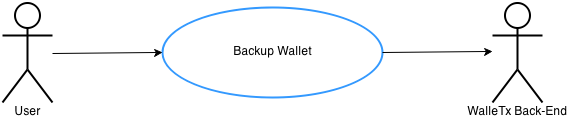
\includegraphics[width=0.6\textwidth]{../diagrams/use-case-backup.png}
      \caption{Backup Data}
    \end{figure}

\begin{table}[H]
  \tabulinesep=1.2mm
      \rowcolors{2}{gray!25}{white}
      \centering
      \resizebox{0.8\columnwidth}{!}{%

      \begin{tabu}{r | X}
        \rowfont{\color{black}}
        \taburulecolor{black}
        \taburowcolors 1{green .. green}

        \multicolumn{2}{l}{\textbf{\textsf{WalleTx: Backup Data}}}\\
        \hline
        \taburowcolors 2{light-gray .. white}

        \textsf{Actors} & User\\
        Description & A user will be able to backup all wallet information, transaction hashes, and tags associate with those transactions to an XML or JSON file.\\
        Data & public wallet identification, transaction hashes, tags associate with transactions\\
        Stimulus & User initiates a data backup\\
        Response & Dialog box will confirm backup\\
        Comments & Is there any additional data that needs to be backed up? Where will the database backup be stored?\\
        \taburowcolors 1{green .. green}
      \multicolumn{2}{|l|}{\textbf{\textsf{\footnotesize{Figure 7.11}}}}\\
      \hline

      \end{tabu}%
    }
    \end{table}

	
    \begin{figure}[H]
      \centering
      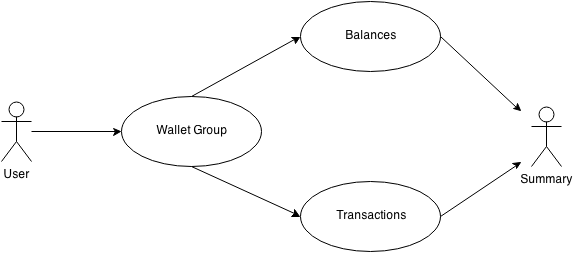
\includegraphics[width=0.8\textwidth]{../diagrams/usecase_3_6.png}
      \caption{Wallet Summary View}
    \end{figure}

\begin{table}[H]
  \tabulinesep=1.2mm
      \rowcolors{2}{gray!25}{white}
      \centering
      \resizebox{0.8\columnwidth}{!}{%

      \begin{tabu}{r | X}
        \rowfont{\color{black}}
        \taburulecolor{white}
        \taburowcolors 2{green .. green}
        \multicolumn{2}{l}{\textbf{\textsf{WalleTx: Wallet Group Summary View}}}\\
        \hline
        \taburowcolors 2{light-gray .. white}
        \textsf{Actors} & User\\
        Description & A user will be able to view a summary of all balances and transactions from created groups.\\
        Data & transactions and current balances within the wallet groups.\\
        Stimulus & User initiates summary view.\\
        Response & A detailed summary is presented to the user.\\
        Comments & The details can be refreshed as often as requested by the user.\\
        \taburowcolors 1{green .. green}
        \multicolumn{2}{|l|}{\textbf{\textsf{\footnotesize{Figure 7.12}}}}\\
      \end{tabu}%
    }
    \end{table}
	
   % \begin{figure}[H]
   %   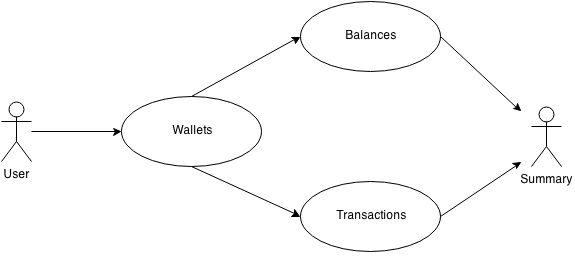
\includegraphics[width=1.0\textwidth]{../diagrams/usecase_3_7.png}
   % \end{figure}

\begin{table}[H]
  \tabulinesep=1.2mm
      \rowcolors{2}{gray!25}{white}
      \centering
      \resizebox{0.8\columnwidth}{!}{%
      \begin{tabu}{r | X}
        \rowfont{\color{black}}
        \taburulecolor{white}
        \taburowcolors 2{green .. green}
        \multicolumn{2}{l}{\textbf{\textsf{WalleTx: Individual Wallet Summary View}}}\\
        \hline
        \taburowcolors 2{light-gray .. white}
        \textsf{Actors} & User\\
        Description & A user will be able to view a summary of all balances and transactions from individual wallets.\\
        Data & transactions and current balances within the wallets.\\
        Stimulus & User initiates summary view.\\
        Response & A detailed summary is presented to the user.\\
        Comments & The details can be refreshed as often as requested by the user.\\
        \taburowcolors 1{green .. green}
        \multicolumn{2}{|l|}{\textbf{\textsf{\footnotesize{Figure 7.12}}}}\\
      \end{tabu}%
    }
    \end{table}

%Identifying use cases:\\
%\begin{itemize}
%\item What are the goals that the actor will attempt to accomplish with the system?
%\item What are the primary tasks that the actor wants the system to perform?
%\item Will the actor create, store, change, remove, or read data in the system?
%\item Will the actor need to inform the system about sudden external changes?
%\item Does the actor need to be informed about certain occurrences, such as unavailability of a network resource, in the system?
%\item Will the actor perform a system startup or shutdown?
%\end{itemize}

%Use cases will be outlined in diagrams provided.\\ 

%The primary task of the customer/user will be to interact with the application.  Their main purpose will be to monitor their bitcoin currency from multiple wallets and tag transactions to better organize all transactions.  The actor will have the ability to add and remove wallets/add and remove tags pertaining to transactions. The actor can observe aggregate information in the form of graphs, charts, etc.  The actor will be alerted to certain trigger events. (updated wallet info, specific transactions, etc).  The actor has the ability to close and open application in running OS and also has the ability to completely remove the application from existing OS. \\
	
	
    \subsubsection{Class Descriptions}
      \begin{figure}[H]
        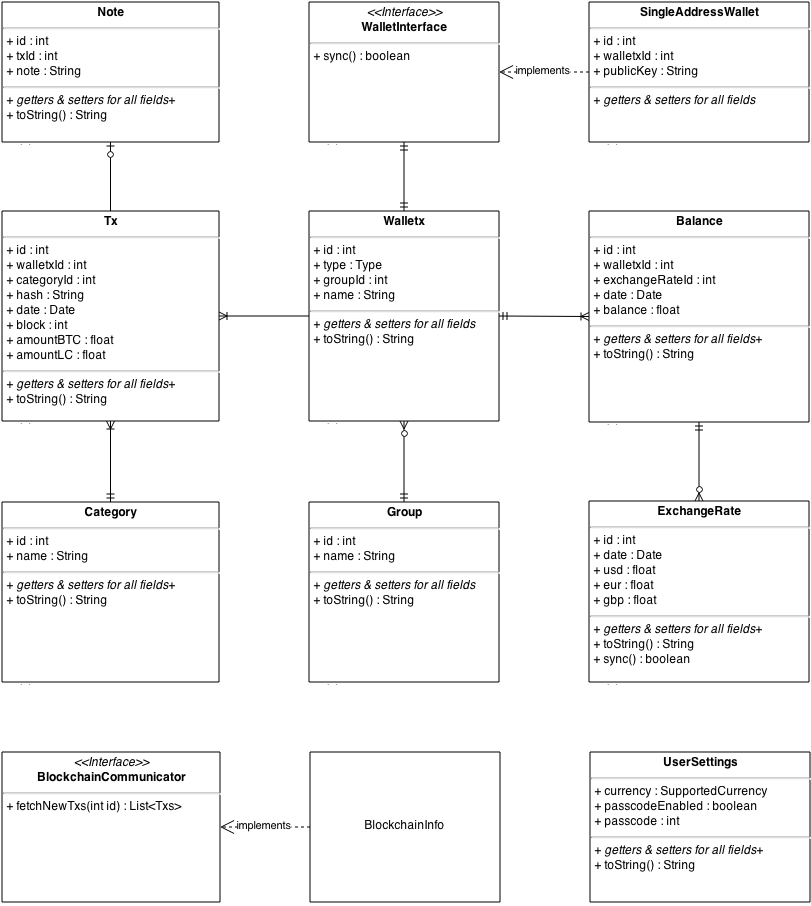
\includegraphics[width=1.0\textwidth]{../diagrams/classes_model.png}
      \end{figure}

    \subsubsection{Attribute Descriptions}
  \subsection{Raw Use Case Point Analysis}
    \subsubsection{Actor Summary Table}
    \begin{table}[H]
      \begin{tabularx}{\textwidth}{r | X}
        Actors                       & Summary\\
        \hline
        Customer/End User            & This actor will be the end user.  They will interact with WalleTx,  providing it with wallet information, tagging transactions, and viewing  aggrated wallet information\\
        Development Team/Maintenance & This actor will be interacting via the support and maintance of the  application.  They will maintain DB orginzation, revision handling, and  overall maintaince of the application\\
        External Bitcoin Wallets     & External Bitcoin Wallets will be providing our application with vital  information.  All external wallets' totals and transactions will  aggregated in WalleTx.\\
        SQLite Database              & This actor is a database stored on each end user's phone. This will  contain data from wallets, transactions, and display information.  It  will interact soley with the application via code.\\
        Bitcoin Blockchain           & The bitcoin blocktrain will provide transaction specific data for all  included wallets. This actor will interact with the application via  database backend.\\
      \end{tabularx}
    \end{table}

    \subsubsection{Use Case Summary Table}
	\begin{table}[H]
      \begin{tabularx}{\textwidth}{r | X}
        Actor                       & Use-Case Summary\\
        \hline
        Customer/End User            & 1. adding a wallet
									   2. removing a wallet
									   3. adding a tag to a transaction
									   4. removing a tag from a transaction
									   5. viewing all wallets
									   6. accessing application settings\\
        Development Team/Maintenance & 1. update revisions
									   2. maintain database structure\\
        External Bitcoin Wallets     & 1. update added wallet information
									   2. provide public key 
									   3. provide transactions made by wallets\\
        SQLite Database              & 1. store wallet data
									   2. wallet data deleted
									   3. wallet data added
									   4. provide data for alerts
									   5. supply data for graphs/charts\\
        Bitcoin Blockchain           & 1. update wallet/DB transactions
									   2. provide data for new wallet added\\
      \end{tabularx}
    \end{table}

    \subsubsection{Screens and Reports with Navigation Matrix}

  \begin{figure}[H]
     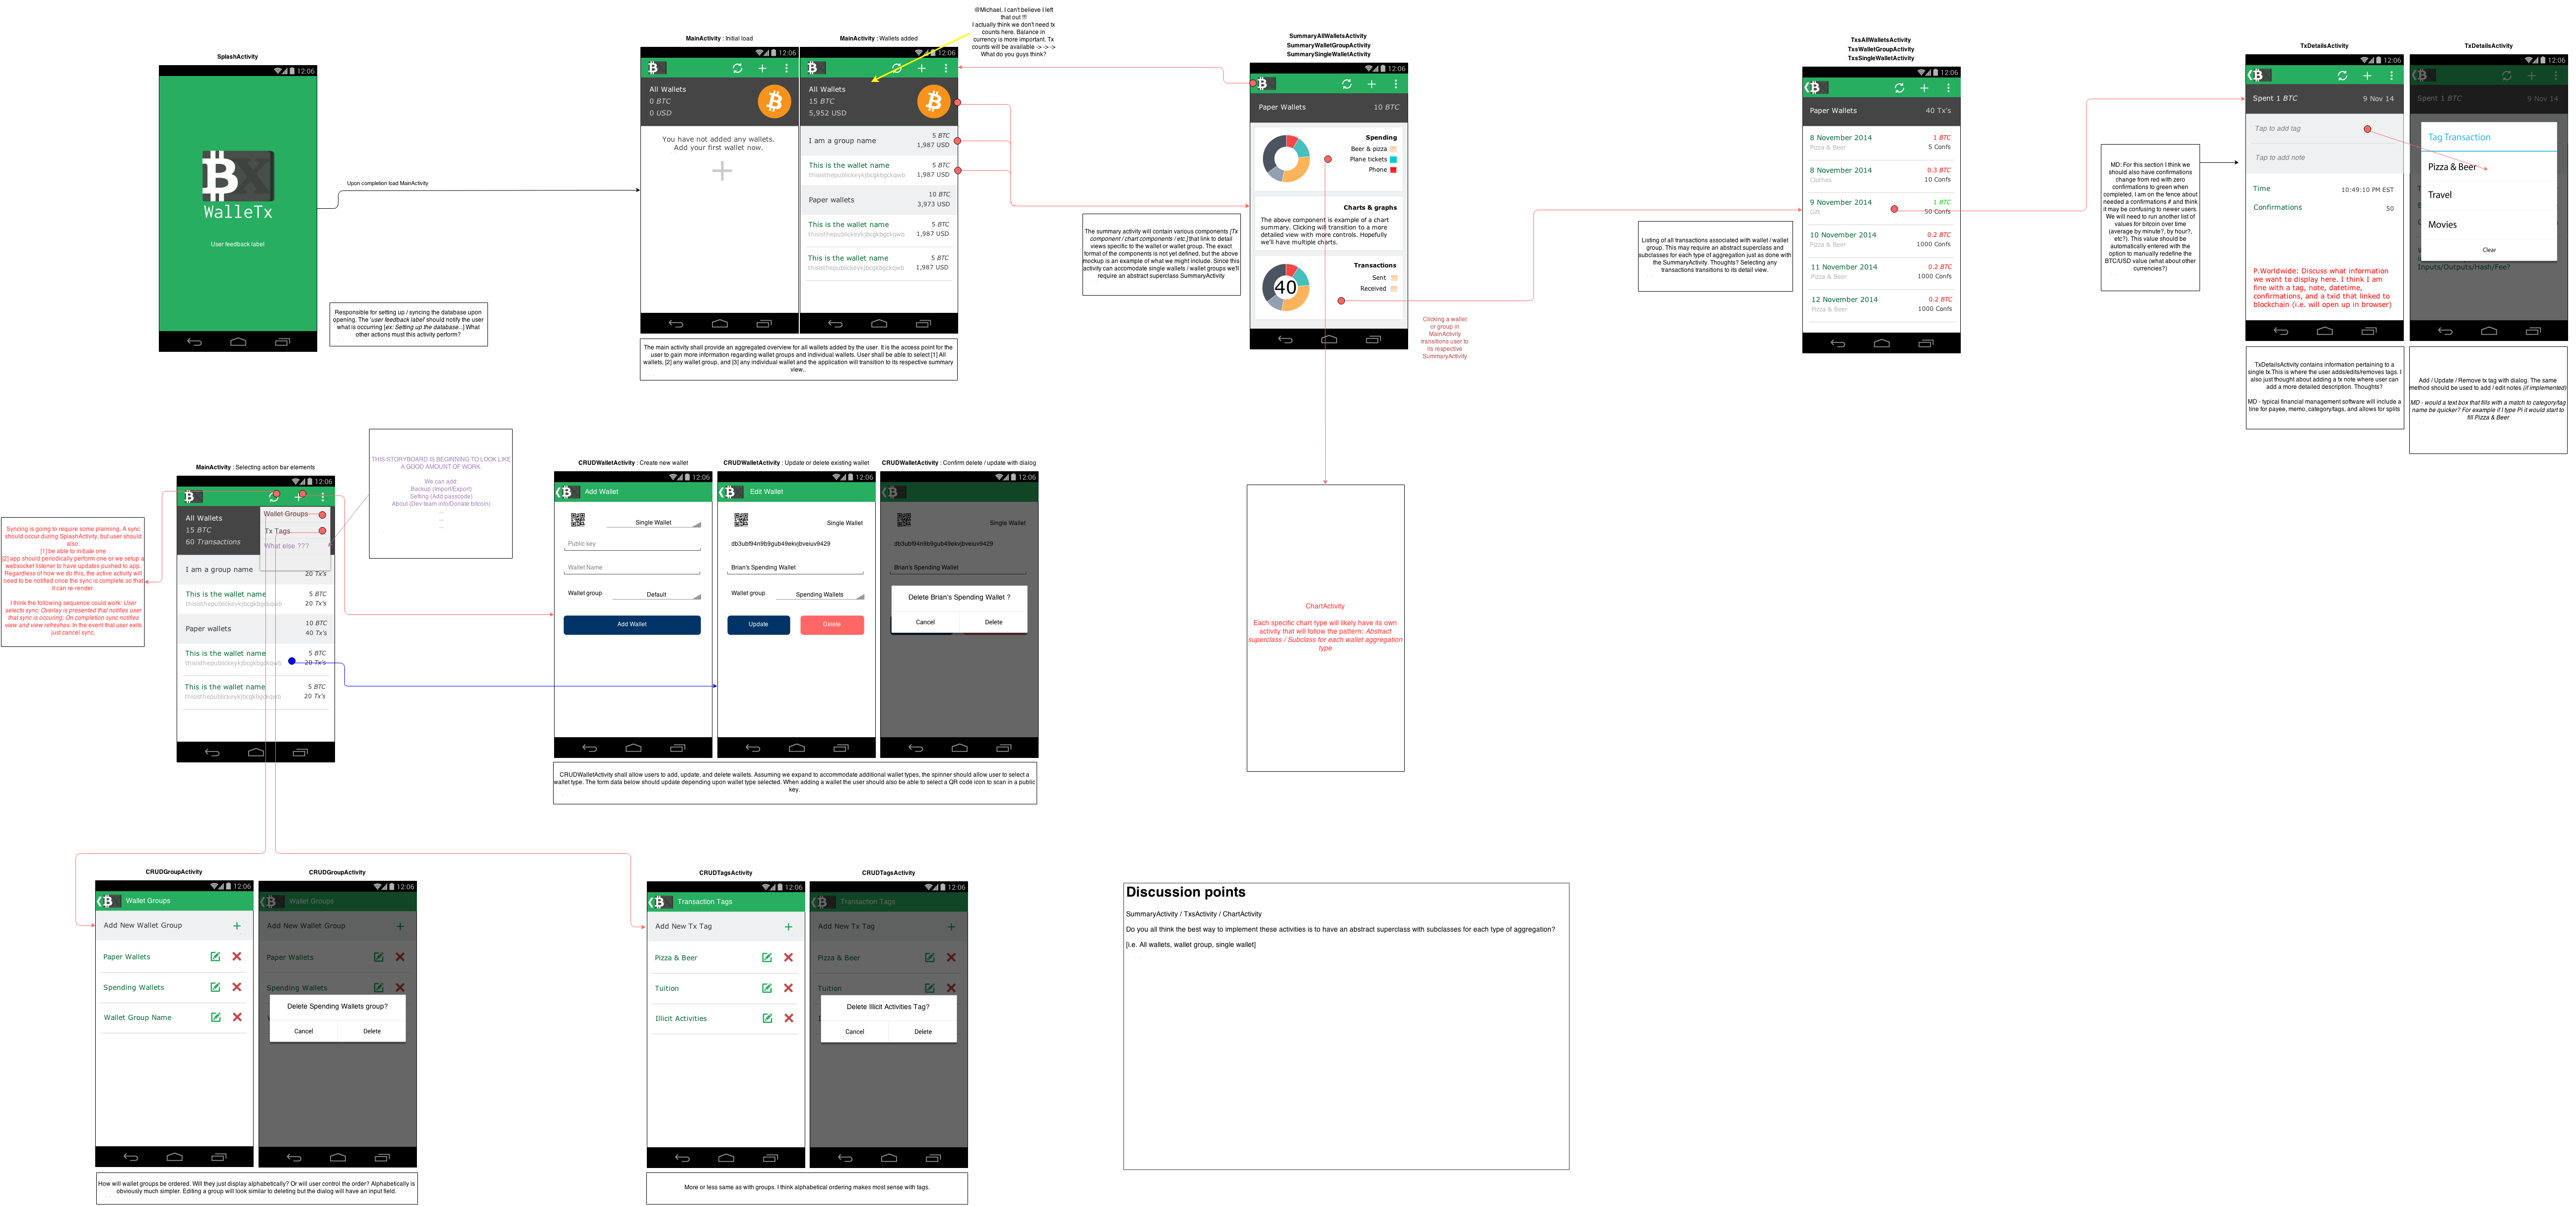
\includegraphics[width=1.0\textwidth]{../diagrams/storyboard_master.png}
  \end{figure}
  \begin{figure}[H]
     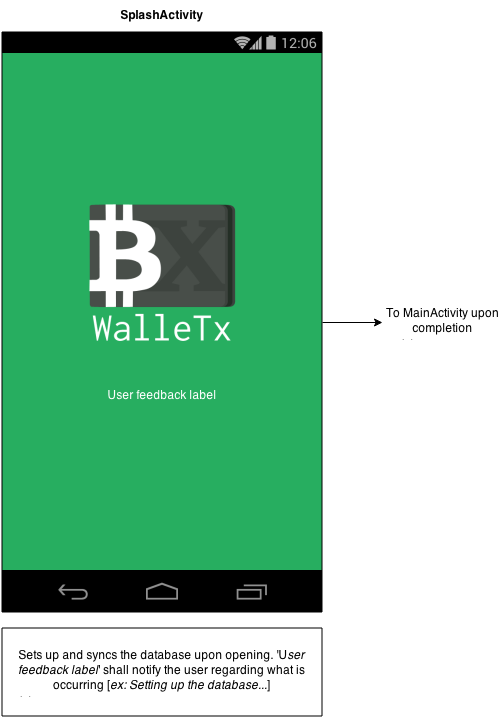
\includegraphics[width=1.0\textwidth]{../diagrams/storyboard_splash.png}
  \end{figure}
	\begin{figure}[H]
     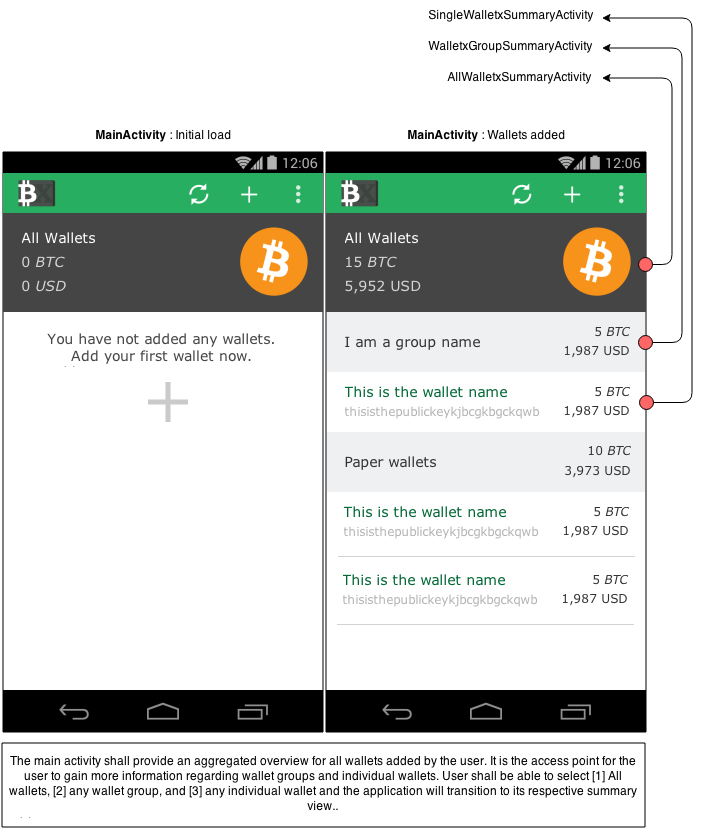
\includegraphics[width=1.0\textwidth]{../diagrams/storyboard_main.png}
  \end{figure}
  \begin{figure}[H]
     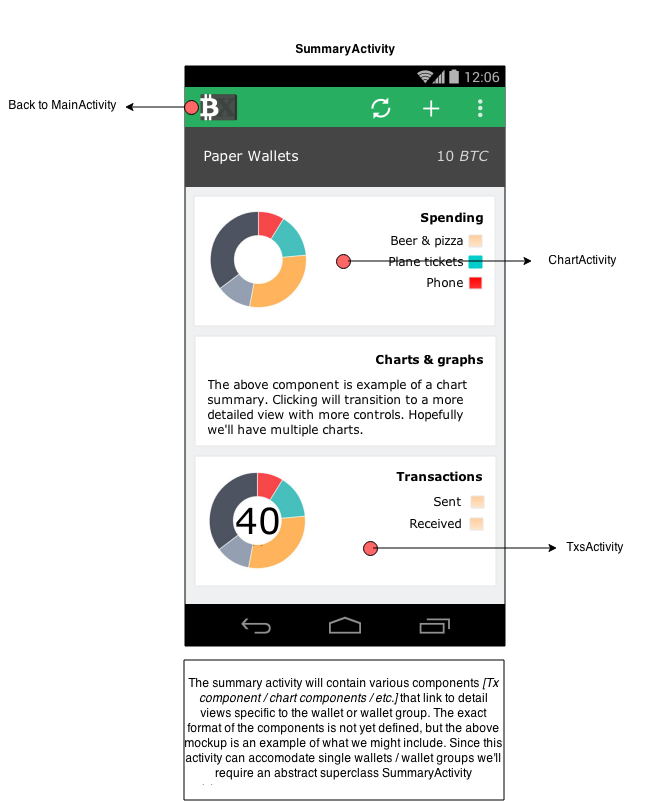
\includegraphics[width=1.0\textwidth]{../diagrams/storyboard_summary.png}
  \end{figure}
  \begin{figure}[H]
    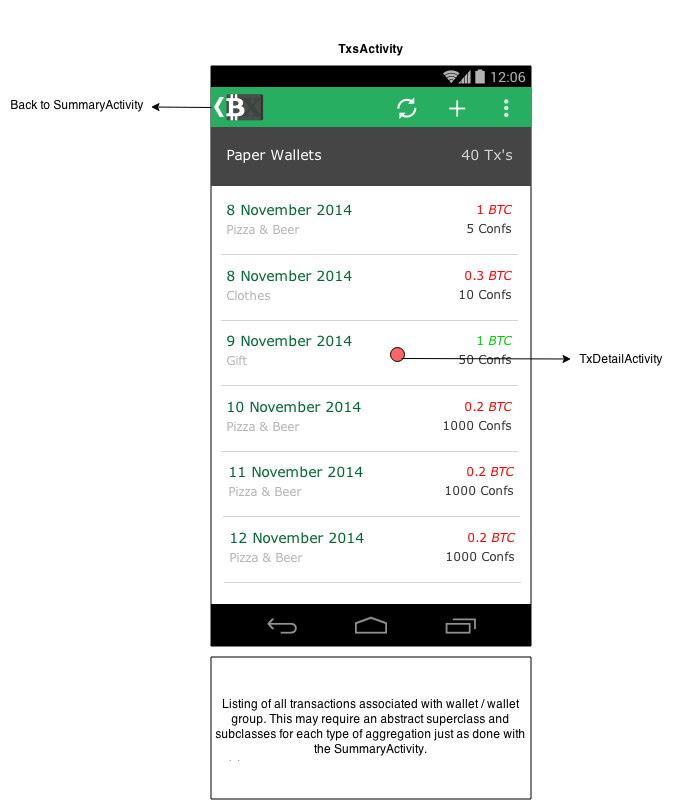
\includegraphics[width=1.0\textwidth]{../diagrams/storyboard_txs.png}
  \end{figure}
  \begin{figure}[H]
    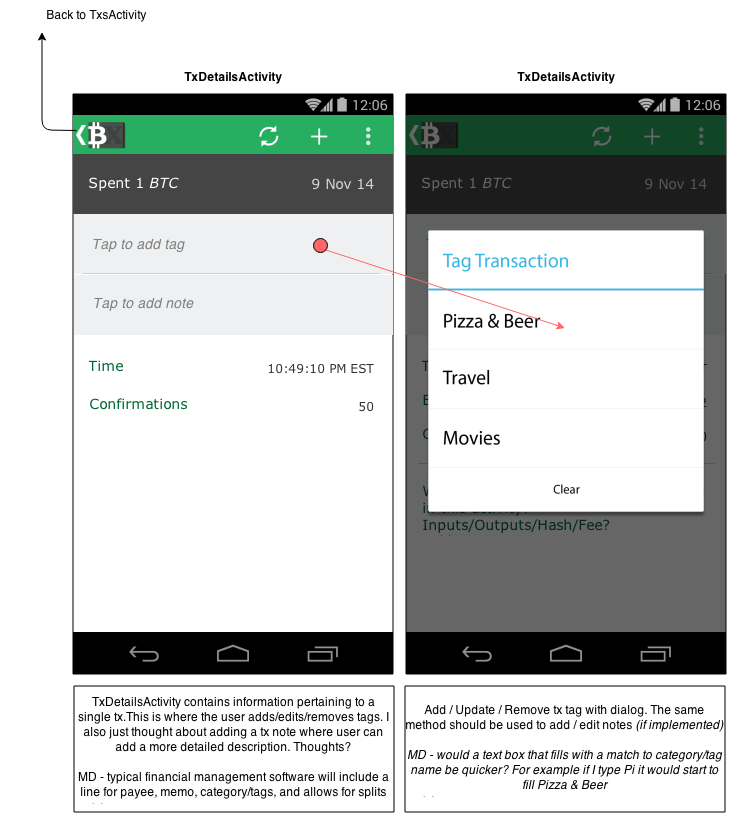
\includegraphics[width=1.0\textwidth]{../diagrams/storyboard_txDetails.png}
  \end{figure}
  \begin{figure}[H]
    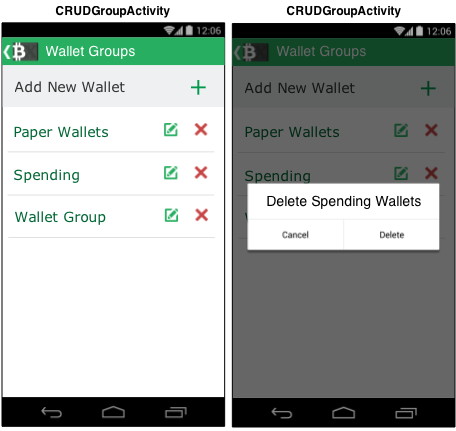
\includegraphics[width=1.0\textwidth]{../diagrams/storyboard_CRUDgroupTag_1.png}
  \end{figure}
  \begin{figure}[H]
    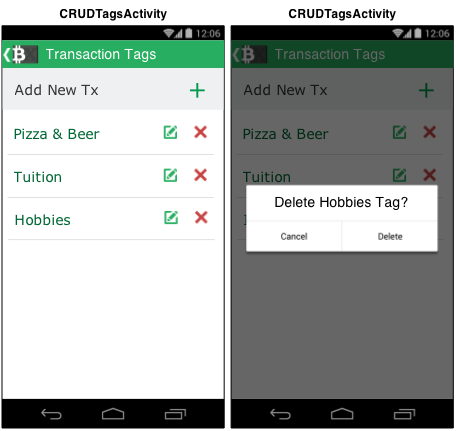
\includegraphics[width=1.0\textwidth]{../diagrams/storyboard_CRUDgroupTag_2.png}
  \end{figure}

  \begin{figure}[H]
     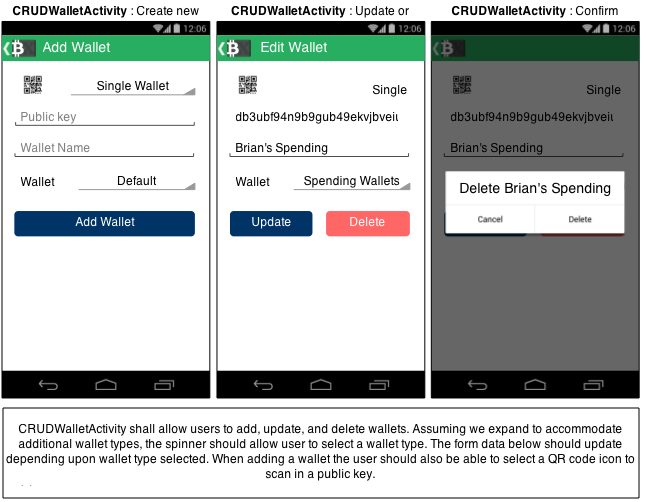
\includegraphics[width=1.0\textwidth]{../diagrams/storyboard_CRUDwallet.png}
  \end{figure}
  
	*Need to create navigation matrix
	*Need to create Reports
	
  \subsection{Other Appendices}
  * will be discussed in next meeting 11/24/2014
